\section{Case Study 2}

Weixin and Haoyuan.

Talk about the 3 case studies

Talk about Pretty Printer case study last and discuss issues with
extensible transformations.

\subsection{Scans}
% statistics, pictures, implementation
The first case study re-implements ?, which is discussed quite thoroughly in
Section~\ref{}.
We strictly follows the flow of the paper and introduce all kinds of
interpretations modularly.
Starting from a plain AST without any interpretations in the base family, we gradually add
\texttt{depth}, \texttt{width}, \texttt{wellSized}, \texttt{layout} and
\texttt{tlayout} methods through extending the family.

The following shows the client code:
\begin{lstlisting}
Circuit circuit =
  above(beside(fan(2), fan(2)),
  above(stretch(fan(2),2,2),
  beside(id(1), beside(fan(2), id(1)))));
\end{lstlisting}

To simplify client code, we defined wrappers around \texttt{of} methods
for conveniently constructing circuits. For instance, the wrapper for
\texttt{Fan} is defined as follows:
\begin{lstlisting}
static Fan fan(int n) {
  return Fan.of(n);
}
\end{lstlisting}
The \texttt{circuit} object supports all the methods stated above.
Additionally, we introduce a \texttt{draw} method which renders a
circuit using Java Swing.
Calling \texttt{draw} on the \texttt{circuit} will
display what Figure~\ref{sec:} shows.

% show Java Swing figure
\begin{figure}
\end{figure}

\subsection{A Prettier Printer}

This case study refactors the Haskell code from \cite{Wadler98aprettier}
which uses deep embeddings to implement a functional pretty printer library with high efficiency. In the original code, two
data structures are defined for documents:
\begin{lstlisting}[keywords={data,Int,String}]
data DOC = NIL
            | DOC :<> DOC
            | NEST Int DOC
            | TEXT String
            | LINE
            | DOC :<> DOC
data Doc = Nil
            | String `Text` Doc
            | Int `Line` Doc
\end{lstlisting}
Here they are encoded with shallow DSLs, and packaged into
two base families with \textsf{@Family} annotation applied. These two families \textsf{Family\_Doc} and
\textsf{Family\_Document} correspond to data types \textsf{Doc} and \textsf{DOC} respectively.

\begin{lstlisting}
@Family interface Family_Doc {
	interface Doc {}
	interface Nil extends Doc {}
	interface Text extends Doc {
		String _s(); Doc _d();
	}
	interface Line extends Doc { int _i(); Doc _d(); }
}

@Family interface Family_Document {
	interface Document {}
	interface DNil extends Document {}
	interface DConcat extends Document {
		Document _d1(); Document _d2();
	}
	interface DNest extends Document {
		int _i(); Document _d();
	}
	interface DText extends Document { String _s(); }
	interface DLine extends Document {}
	interface DUnion extends Document {
		Document _d1(); Document _d2();
	}
}
\end{lstlisting}

With the help of family polymorphism and \textsf{@Family}, we can easily add new operations and integrate them
in child families. Below is an example of encoding two original functions \textsf{layout} and \textsf{fits} in
the shallow embeddings. Note that with the annotation processing, verbose code for building inheritance relations is
automatically generated.
\begin{lstlisting}
@Family interface Family_Doc_LayoutFits extends Family_Doc {
	interface Doc {
		String layout(); boolean fits(int w);
	}
	interface Nil {
		default String layout() { return ""; }
		default boolean fits(int w) {
			return w >= 0;
		}
	}
	...
\end{lstlisting}
Furthermore, the function \textsf{be} needs refactoring before it is encoded in shallow embeddings.
The original \textsf{be} is defined as follows:
\begin{lstlisting}
be w k [] = Nil
be w k ((i,NIL):z) = be w k z
be w k ((i,x :<> y):z) = be w k ((i,x):(i,y):z)
be w k ((i,NEST j x):z) = be w k ((i+j,x):z)
be w k ((i,TEXT s):z) = s `Text` be w (k+length s) z
be w k ((i,LINE):z) = i `Line` be w i z
be w k ((i,x :<|> y):z) = better w k (be w k ((i,x):z)) (be w k ((i,y):z))
\end{lstlisting}
We refactor it by introducing a helper function \textsf{beaux}:
\begin{lstlisting}
beaux w k i NIL z = be w k z
beaux w k i (x :<> y) z = be w k ((i,x):(i,y):z)
beaux w k i (NEST j x) z = be w k ((i+j,x):z)
beaux w k i (TEXT s) z = s `Text` be w (k+length s) z
beaux w k i LINE z = i `Line` be w i z
beaux w k i (x :<|> y) z = better w k (be w k ((i,x):z)) (be w k ((i,y):z))

be w k [] = Nil
be w k ((i,x):z) = beaux w k i x z
\end{lstlisting}
In this case, \textsf{beaux} can be defined as an operation method \lstinline{beaux(int, int, int, List<Pair<int, Document>>)} inside the type \textsf{Document}, and
its pattern matching corresponds to the default implementations in different member types (like \textsf{DNil}, \textsf{DConcat}, etc). On the other hand, \textsf{be} is implemented as a static method
\lstinline{be(int, int, List<Pair<int, Document>>)} outside the member types.

Finally we finished the refactoring of the pretty printer library using a set of extensible families with shallow DSLs and operations, and our
\textsf{@Family} annotation. However there is a special operation called \textsf{group}, which works like a transformation:
\begin{lstlisting}
@Family interface Family_Document_Flatten extends Family_Document {
	interface Document {
		Document flatten();
		default Document group() {
			return DUnion.of(this.flatten(), this);
		}
	}
	...
}
\end{lstlisting}
The method \textsf{group} calls the constructor method from \textsf{DUnion}, whereas such a member type will be updated in the
child families, together with its constructors. To ensure type safety we are unable to reuse the code but just copy it and paste
to the child families, and hence code duplication is introduced by the use of factory methods. The matter of extensible
transformations will be further discussed in the next section.


\subsection{Diagrams}
\emph{diagrams}~\cite{yates2015diagrams} is a declarative Haskell EDSL for creating vector graphics.
This case study implements a simplified version of \emph{diagrams} from
Gibbons's lecture notes~\cite{gibbonsexercises}.

\subsubsection{The Language}
The DSL consists of three simpler sub-languages for describing shapes, styles
and pictures. Note that all these definitions are put inside a base family.

% Haskell code
\begin{comment}
\begin{lstlisting}[language=haskell]
data Shape
  = Rectangle Double Double
  | Ellipse Double Double
  | Triangle Double

type StyleSheet = [Styling]
data Styling
  = FillColour Col
  | StrokeColour Col
  | StrokeWidth Double

data Col = Red | Blue | Bisque | Black | Green | Yellow | Brown

data Picture
  = Place StyleSheet Shape
  | Above Picture Picture
  | Beside Picture Picture
\end{lstlisting}
\end{comment}

\paragraph{Shapes}
Shapes are fundamental components of a picture. The sub-language provides three
primitives for constructing rectangles, ellipses and triangles:

\lstinputlisting[linerange=111-120]{./src/diagrams/Diagrams.java}%APPLY:SHAPE

\paragraph{Styles}
A shape can be decorated with drawing styles. A \texttt{StyleSheet} contains a
list of \texttt{Stylings} for specifying fill color, stroke color or stroke width:

\lstinputlisting[linerange=124-136]{./src/diagrams/Diagrams.java}%APPLY:STYLE
\lstinputlisting[linerange=140-145]{./src/diagrams/Diagrams.java}%APPLY:COLOR

The definition of \texttt{StyleSheet} reveals how to deal with lists or more generally
collection types in \name. We capture the element type using a wildcard with an upper
bound (\texttt{? extends Styling}) to model covariant lists. This allows the
upper bound to be refined with its subtype in extensions. As a result, we are
able to invoke new interpretations on elements of the list.


\paragraph{Pictures}
Provided with a \texttt{StyleSheet}, a \texttt{Shape} can be lifted to a
\texttt{Picture} using \texttt{Place}. Meanwhile, two pictures can be
combined together vertically or horizontally via binary combinator
\texttt{Above} and \texttt{Beside} respectively:

\lstinputlisting[linerange=151-160]{./src/diagrams/Diagrams.java}%APPLY:PICTURE

We can already draw simple pictures based on existing definitions.
For example, Figure~\ref{woman} (with auxiliary wrappers defined) shows
a woman in a red dress and blue stockings.
To actually visualize the picture as shown in the right hand side of
Figure~\ref{woman}, we need to give semantics to the language for animation.

\begin{figure*}
  \begin{tabular}{lr}
\begin{minipage}[t]{.9\textwidth}
\lstinputlisting[linerange=537-544]{./src/diagrams/Diagrams.java}%APPLY:WOMAN
\end{minipage}
&
\begin{minipage}[t]{.1\textwidth}
  \vspace{0.2em}
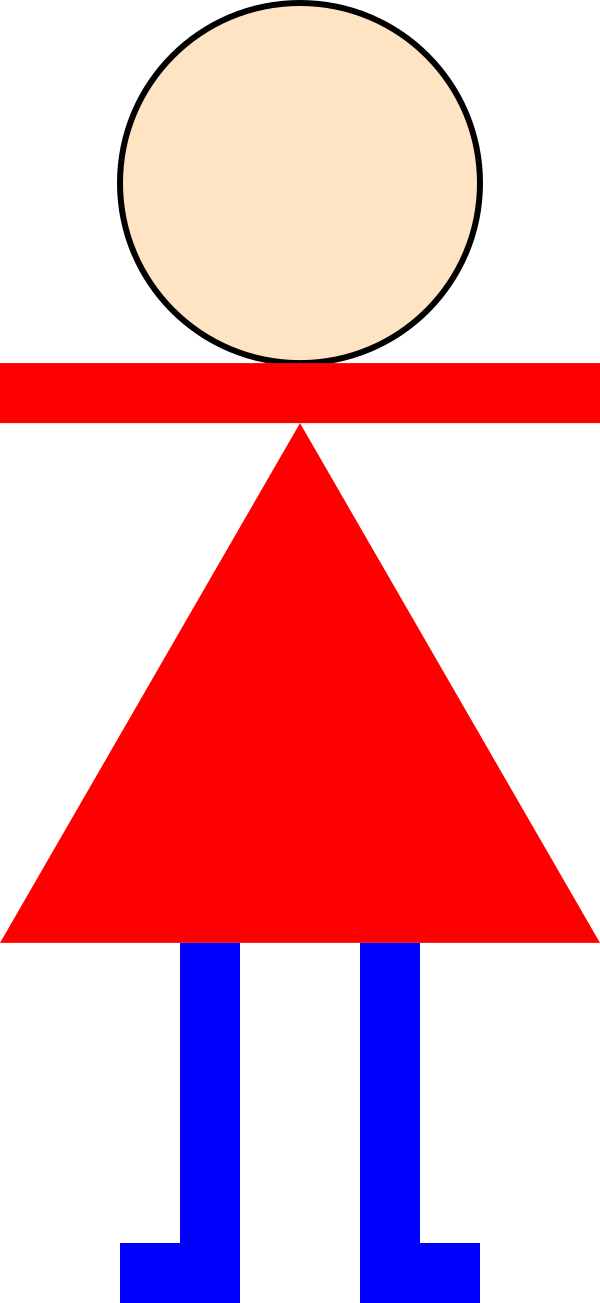
\includegraphics[width=1.3cm]{woman.png}
\end{minipage} \\
\end{tabular}
\caption{A woman drawn in \emph{diagrams}}
\label{woman}
\end{figure*}

\subsubsection{Animation}
We use scalable vector graphics (SVG) as the backend for rendering
pictures.
SVG aligns styled shapes by center, which requires us to determine a center
point of a picture as the origin of coordinate, and calculate
positions of all the shapes inside the picture accordingly.
To represent a position in the coordinates we define \texttt{Pos}:
\begin{lstlisting}
@Obj interface Pos {
    double _x(); double _y();
}
\end{lstlisting}
The position of a shape can then be determined by a pair of \texttt{Pos}, called
an extent,
locating the lower left and upper right conners:
\begin{lstlisting}
@Obj interface Extent {
    Pos _p1(); Pos _p2();
}
\end{lstlisting}
These definitions are stable so we put them out of the family and annotated
with \texttt{@Obj}.

Given an individual shape, its extent can be calculated according to its type.
We therefore extend \texttt{Shape} with a \texttt{toExtent} method:

\begin{lstlisting}
    interface Shape {
        Extent toExtent();
    }
\end{lstlisting}

When pictures are combined together, the center point is changed and hence the
positions of shapes in both pictures should all be recalculated.
The transformation sub-language records how to adjust those positions,
which includes identity transformation, translations, and compositions of the two:

\lstinputlisting[linerange=164-171]{./src/diagrams/Diagrams.java}%APPLY:TRANSFORM

\paragraph{Drawing}
To easily translate a \texttt{Picture} into SVG format, we flatten the recursively structured pictures into a non-empty
sequence of transformed styled shapes, represented by \texttt{Drawing}:

\begin{lstlisting}
interface Drawing {
    List<? extends Shape> _shapes();
    List<? extends StyleSheet> _styles();
    List<? extends Transform> _transforms();
}
\end{lstlisting}

% Step 1: Picture to Drawing
To generate a \texttt{Drawing} from a \texttt{Picture}, we extend the
\texttt{Picture} hierarchy with a \texttt{draw} method:
\lstinputlisting[linerange=279-281]{./src/diagrams/Diagrams.java}%APPLY:DRAW

% The implementation for each case is omitted here for space reasons.

% Step 2: Drawing to XML
With all the necessary information contained in drawing, we can now generate the
SVG file. SVG is based on XML and the structure of an XML file can be captured by following definitions:
\begin{lstlisting}
@Obj interface XML {
    String _tag();
    List<Attr> _attrs();
    List<XML> _xmls();
}
@Obj interface Attr {
    String _name(); String _value();
}
\end{lstlisting}
We then extend a \texttt{toXML} method both in \texttt{Drawing} and \texttt{Shape}.
\begin{lstlisting}
interface Shape {
  XML toXML(List<Attr> styleAttrs, Transform trans);
}
interface Drawing {
  XML toXML();
}
\end{lstlisting}
Calling \texttt{toXML} on a \texttt{Drawing} will builds up a complete XML by calling the \texttt{toXML} on each \texttt{Shape}.

The final step is to pretty print the content of an \texttt{XML} object and
save it to an file with the extension \emph{svg}.
Then open the file with a modern browser, you will see the right side of
Figure~\ref{woman} appear on the screen.

\subsubsection{Discussion}
Each sub-language retains independent extensibility.
\cite{} contains exercises about extensions on the language, e.g.
adding new shapes.
The deep embedding approach in Haskell requires modifications on the ADTs
whereas our approach can modularly introduce new language constructs.
At the same time, new interpretations can be added modularly.
For example, we can add a \texttt{show} method for the purpose of debugging.
